\documentclass{beamer}
\usetheme{Luebeck}
\usecolortheme{beaver}
\setbeamertemplate{navigation symbols}{}

\usepackage{multimedia}
\usepackage{graphicx} 
\usepackage{animate}
\usepackage{multicol}
\usepackage{cite}
\usepackage[utf8]{inputenc}
\usepackage[ngerman]{babel}
\usepackage{tikz}
\usetikzlibrary{calc}

\definecolor{pbfill}{HTML}{FF6960}% filling color for the progress bar
\definecolor{pbbg}{HTML}{575757}% background color for the progress bar

\makeatletter
\newcommand\progressbar@progressbar{} % the progress bar
\newcount\progressbar@tmpcounta% auxiliary counter
\newcount\progressbar@tmpcountb% auxiliary counter
\newdimen\progressbar@pbht %progressbar height
\newdimen\progressbar@pbwd %progressbar width
\newdimen\progressbar@tmpdim % auxiliary dimension

\progressbar@pbwd=\paperwidth
\progressbar@pbht=0.5ex
\newcommand\progressbar@ffn{1}% Anzahl frames für Titelseite und 


% add page numbering
\expandafter\def\expandafter\insertshorttitle\expandafter{%
	\insertshorttitle\hfill%
	\hspace{40px}\insertframenumber\,/\,\inserttotalframenumber}

% the progress bar
\def\progressbar@progressbar{%
	\ifnum\insertframenumber>\progressbar@ffn
	
	\progressbar@tmpcounta=\insertframenumber
	\advance\progressbar@tmpcounta by -\progressbar@ffn
	\progressbar@tmpcountb=\inserttotalframenumber
	\advance\progressbar@tmpcountb by -\progressbar@ffn
	\progressbar@tmpdim=\progressbar@pbwd
	\multiply\progressbar@tmpdim by \progressbar@tmpcounta
	\divide\progressbar@tmpdim by \progressbar@tmpcountb
	
	\begin{tikzpicture}
		
	%%\shade[top color=pbbg!20,bottom color=pbbg!20,middle color=pbbg!20]
	\path[fill=pbbg!20]
	(0pt, 0pt) rectangle ++ (\progressbar@pbwd, \progressbar@pbht);
	
	%%\shade[draw=pbfill,top color=pbfill!50,bottom color=pbfill!50,middle color=pbfill] 
	\path[fill=pbfill!70]
	(0pt, 0pt) rectangle ++ (\progressbar@tmpdim, \progressbar@pbht);
	
	\end{tikzpicture}%
	\fi%
}

\addtobeamertemplate{footline}
{%
	\begin{beamercolorbox}[wd=\paperwidth,ht=3ex,center,dp=0ex]{white}%
		\progressbar@progressbar%
	\end{beamercolorbox}%
}{}
\makeatother
%#####


\title{Fouriertransformation -- Abtasttheorem}
\author{Steffen Walter (1145690) \ Marvin Gaube (4670273)}
\institute{Duale Hochschule Baden-Württemberg -- Stuttgart\newline Vorlesung: Digitale Bildverarbeitung}
\centering
\date{16. April 2020}
\begin{document}
	\maketitle
	\begin{frame}{Agenda}
		\section{Agenda}
		\begin{enumerate}
			\item Theoretische Grundlagen
			\item Praktische Anwendung
			\item Realisierung
			\begin{itemize}
				\item Platzhalter
			\end{itemize}
			\item Fazit
		\end{enumerate}
	\end{frame}

	
	\begin{frame}{Theoretische Grundlagen}
	\section{Theoretische Grundlagen}
	%	Die Digitalisierung eines kontinuierlichen Bildes bedeutet einen enor-
	%	men Datenverlust, da wir die kontinuierliche Grauwertinformation auf
	%	eine Funktion auf einem Raster von Punkten reduzieren. Es stellt sich al-
	%	so die entscheidende Frage, unter welchen Bedingungen wir sicherstellen
	%	können, dass die Abtastpunkte das kontinuierliche Bild realitätsgetreu,
	%	also ohne Informationsverlust, wiedergeben. Zusätzlich interessiert uns,
	%	wie sich ein kontinuierliches Bild aus den Abtastpunkten rekonstruieren
	%	lässt.
	\nocite{bildverarbeitung}
	\begin{itemize}
		\item Platzhalter
	\end{itemize}
	\end{frame}

	\begin{frame}{Abtastung}
	\begin{itemize}
		\item Abtastung bedeutet, dass nur die Information an den Gitterpunkten erhalten bleibt
		\item Mathematisch ist dies eine Multiplikation mit einer Funktion, die nur an den Gitterpunkten ungleich null ist
		\item Diese Operation lässt sich durchführen, indem wir die Bildfunktion $g(x)$ mit einer Funktion multiplizieren, welche die Summe der an den Gitterpunkten $r_{m,n}$ sitzenden $\delta$-Funktionen darstellt
		\item Diese Funktion wird in der Literatur oft als Nagelbrettfunktion oder 2D-$\delta$-Kamm bezeichnet
	\end{itemize}
	
	\end{frame}

	\begin{frame}{Abtastung}
	\begin{itemize}
		\item Eine dichte Abtastung im x-Raum führt zu einem weiten Gitter im k-Raum und umgekehrt. Damit führt die Abtastung zu einer Wiederholung des Bildspektrums an jedem Gittervektor im Fourierraum.
		\item Es folgt, dass die Abtastung zu einer Reduktion der Auflösung führt, d. h., dass Strukturen von der Größe der Abtastschrittweite oder kleiner verloren gehen.
	\end{itemize}
	
	\end{frame}

	\begin{frame}{1D Aliasing-Effekt}
	\begin{block}{Beschreibung}
		Bei der Abtastung eines Signals mit einer Abtastfrequenz etwas kleiner als die Wellenlänge kommt es zum Aliasing-Effekt. Aus dem hochfrequenten Signal wird ein deutlich niederfrequenteres Signal abgetastet. 
	\end{block}
	
	\begin{figure}
		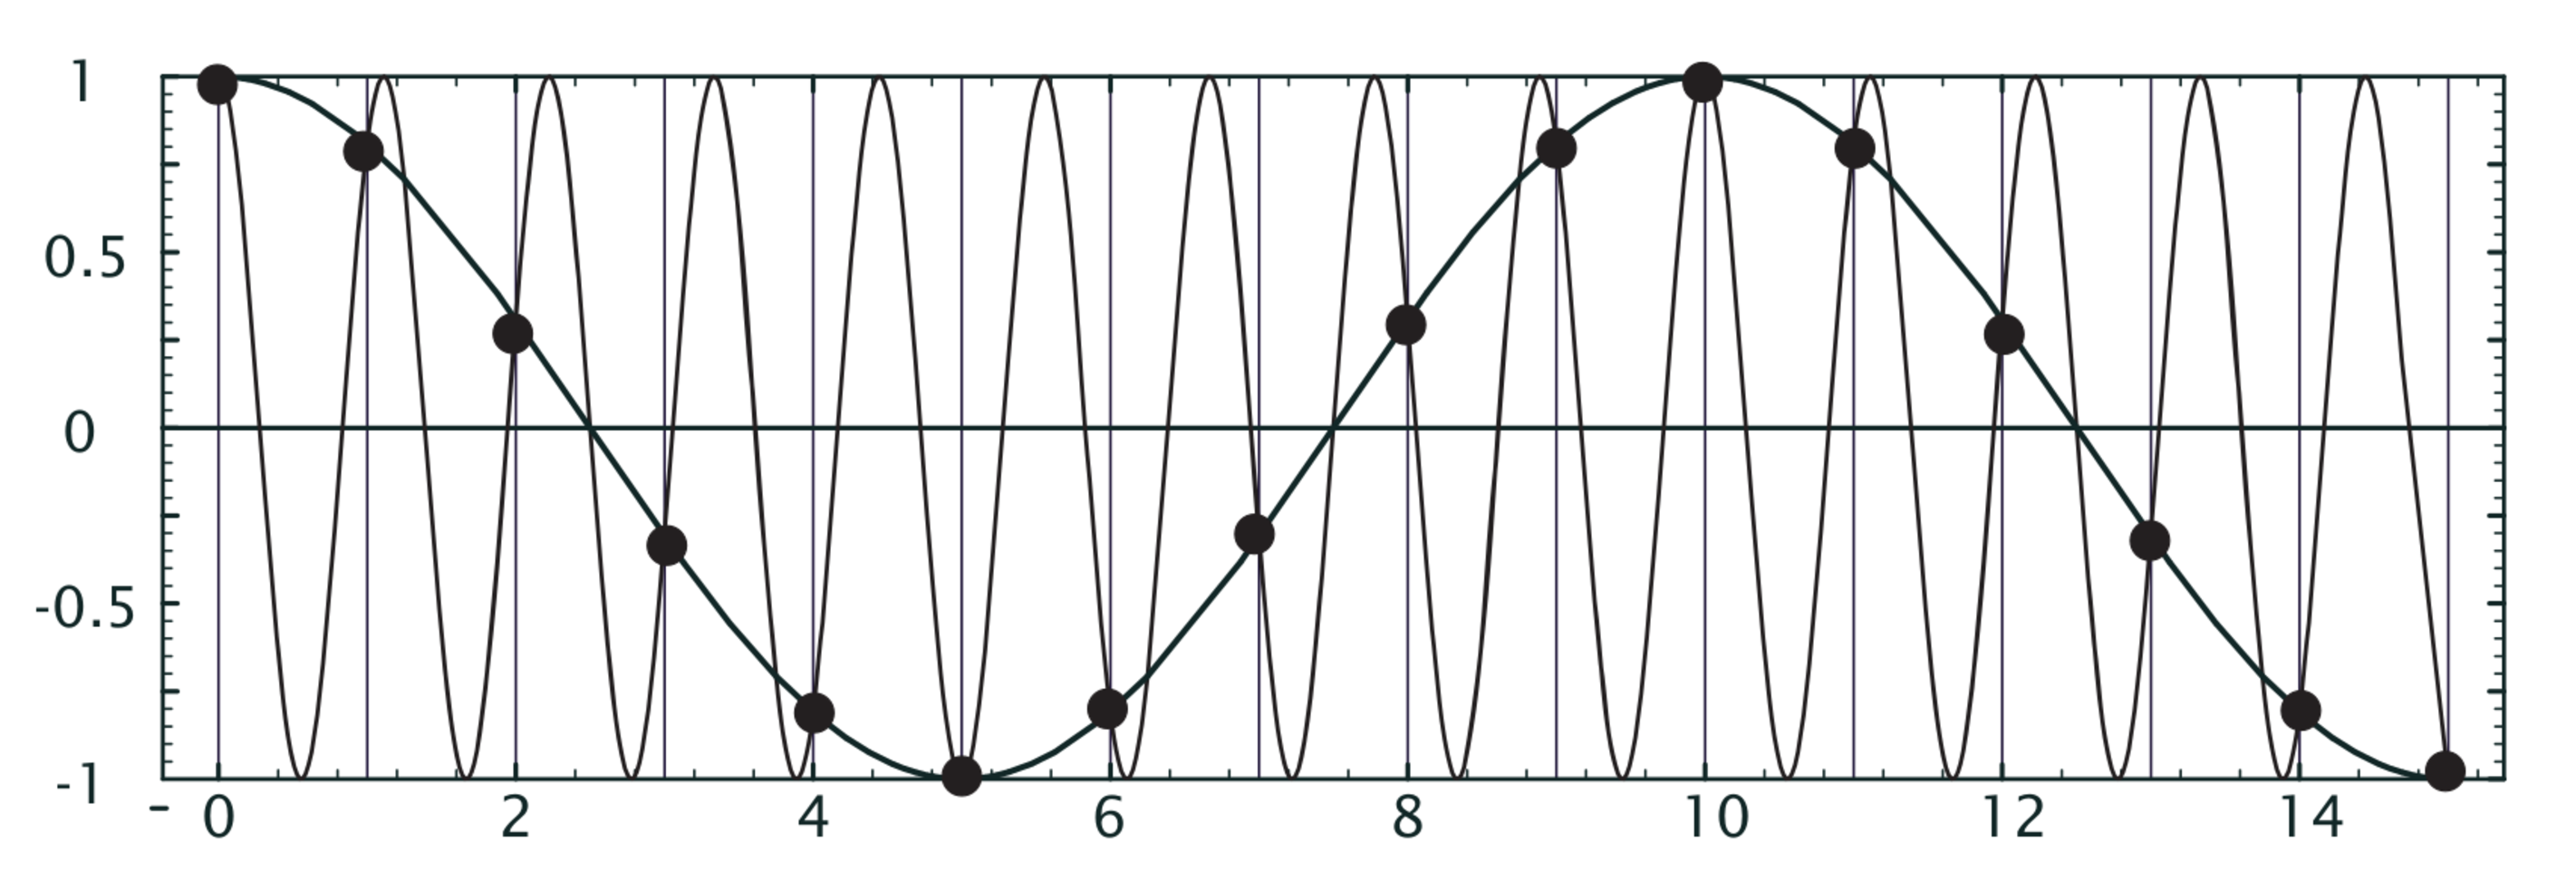
\includegraphics[width=\textheight]{antialiasing.pdf}
		\caption{\footnotesize Veranschaulichung des Aliasing-Effektes. Quelle\cite{bildverarbeitung}}
	\end{figure}
	
	\end{frame}

	\begin{frame}{1D Abtasttheorem}
	\begin{block}{Beschreibung}
		Das Abtasttheorem formuliert die Bedingung, welche nötig ist um eine Verfälschung des Signals bei der Abtastung zu vermeiden:
	\end{block}
	\begin{multicols}{2}
		
	
	\begin{itemize}
		\item Aus Abbildung ergibt sich $(f_p-f_g)-f_g \ge 0$
		\item Daraus lässt sich folgendes Ableiten: $f_p \ge 2f_g$
		\item $f_p$ ist hierbei die Abtastfrequenz 
	\end{itemize}
	
	\begin{figure}
		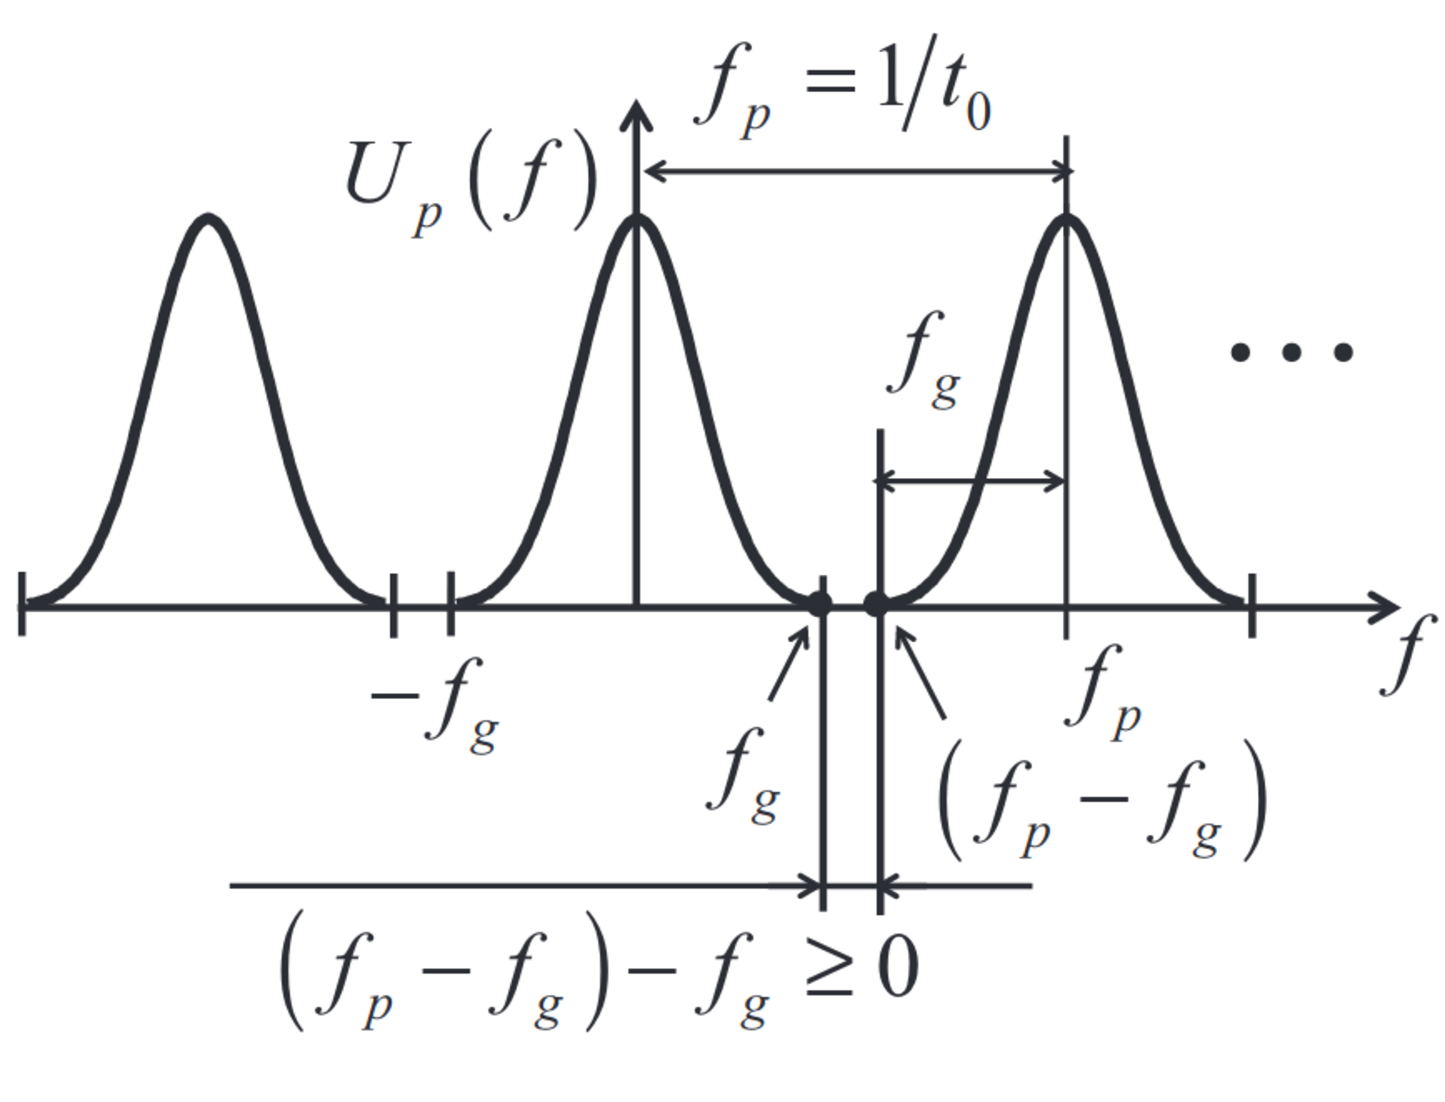
\includegraphics[width=0.58\textheight]{abtasttheorem.pdf}
		\caption{\footnotesize Bedingungen Abtasttheorem. Quelle\cite{lange}}
	\end{figure}
	\end{multicols}
	\end{frame}

	\begin{frame}{2D Aliasing-Effekt}
	\framesubtitle{Moiré-Effekt}
	\begin{figure}
		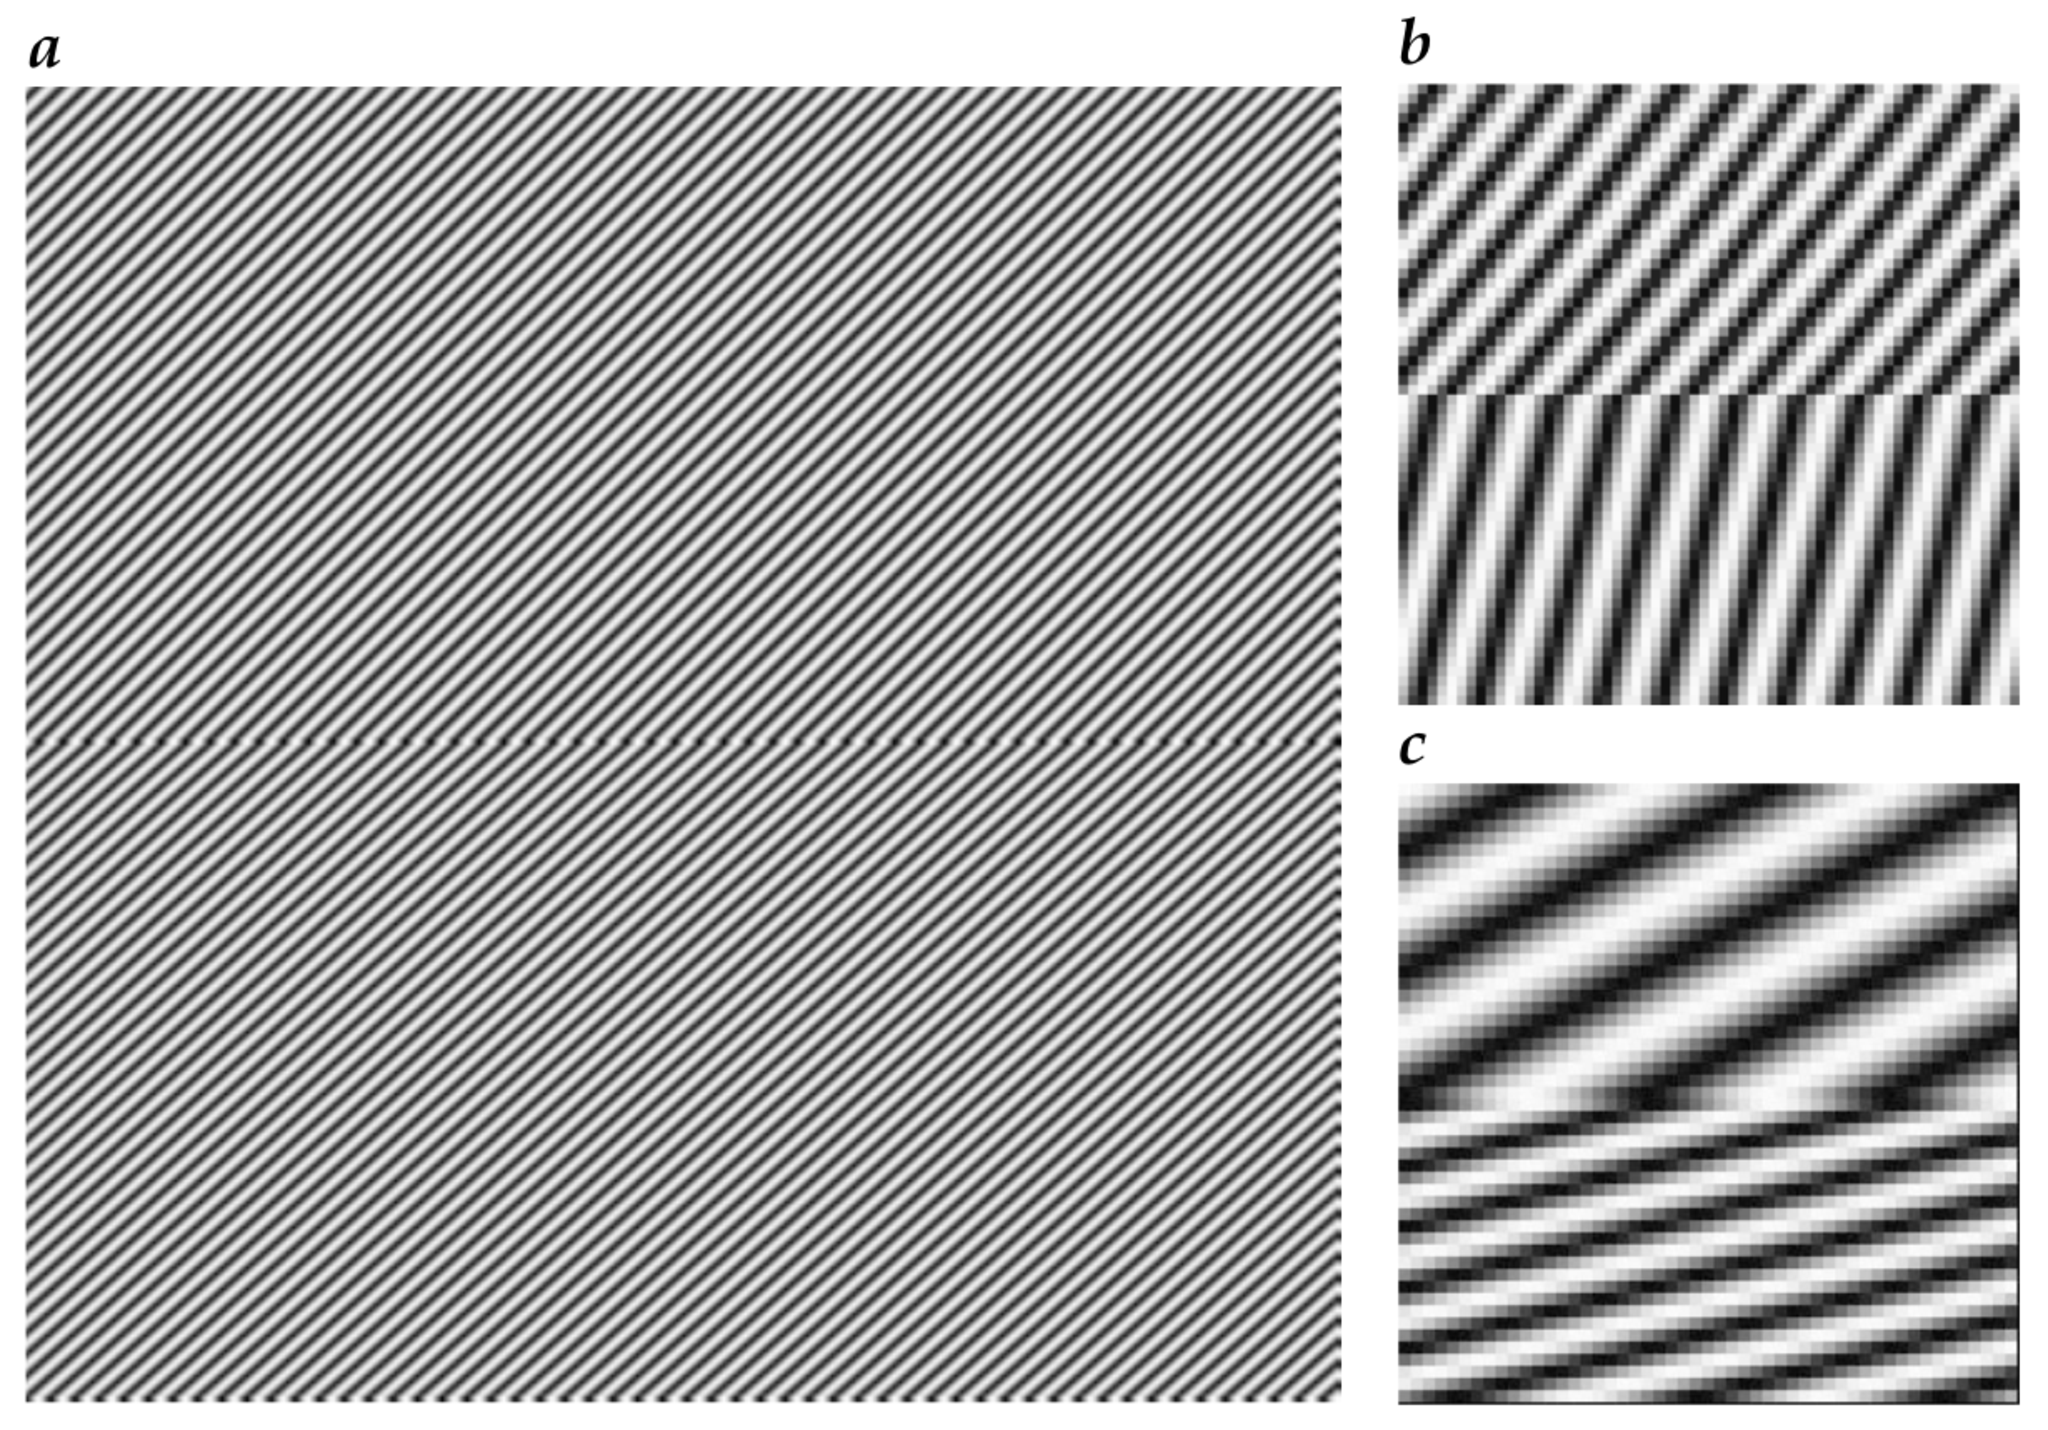
\includegraphics[width=0.7\textheight]{moire.pdf}
		\movie[height=3.5cm, width=5cm, poster, loop]{}{moire.mpg}
		\caption{\footnotesize Der Moiré-Effekt: \textbf{a} Originalbild mit zwei periodischen Mustern (oben $\hat{k} = [0.21, 0.22]^T$ , unten $\hat{k} = [0.21, 0.24]^T$ ). \textbf{b} Jeder vierte und \textbf{c} jeder fünfte Punkt in jeder	Richtung abgetastet. Quelle 1 (links)\cite{bildverarbeitung} Quelle 2 (rechts) \href{https://upload.wikimedia.org/wikipedia/en/4/42/Moir\%C3\%A9.gif}{Internet-Link}}
	\end{figure}
	\end{frame}

	\begin{frame}{2D Abtasttheorem}
	\begin{itemize}
		\item Bei einem großen Bildspektrum können wir nicht vermeiden, dass es Überlappungen von Frequenzen gibt.
		\item Wir können in diesen Fällen keine automatisierte Entscheidung treffen, welche Frequenz der korrekten Darstellung entspricht.
		\item  Um Verzerrungen zu vermeiden, müssen wir Überlappungen ausschließen.
		\item Wir müssen das Spektrum auf den Bereich um den zentralen Punkt des reziproken Gitters bis zu den Linien, die den Zentralgitterpunkt von allen anderen Gitterpunkten trennen, beschränken.
	\end{itemize}
	\end{frame}

	\begin{frame}{2D Abtasttheorem}
	\begin{itemize}
		\item Auf einem Rechteckgitter ergibt sich daraus die einfache Bedingung,	dass die maximale Wellenzahl, bei der das Bildspektrum nicht null ist,
		auf weniger als die Hälfte der Gitterkonstanten des reziproken Gitters beschränkt werden muss.
		\item Quantitativ kann das so ausgedrückt werden: Ist das Spektrum $\tilde{g}(\kappa)$ einer kontinuierlichen Funktion $g(x)$ bandbegrenzt, d. h.
		$$
		\tilde{g}(\kappa) = 0 \forall \left\|k_d\right\|\ge \frac{k_d}{2}
		$$
		dann kann es aus Punkten welche mit der Schrittweite
		$$
		\Delta x_d = \frac{1}{k_d}
		$$
		abgetastet wurde exakt rekonstruiert werden.
	\end{itemize}
	\end{frame}


	\begin{frame}{Praktische Anwendung}
	\framesubtitle{Wo kommt das Abtasttheorem zum Einsatz?}
	\section{Praktische Anwendung}
	\end{frame}
	
	\begin{frame}{Realisierung}
	\framesubtitle{Implementierung in MATLAB}
	\section{Realisierung}	
	\end{frame}

	\begin{frame}{Fazit}
	\section{Fazit}
	\begin{itemize}
		\item Platzhalter
	\end{itemize}
	\end{frame}
	
	\begin{frame}{Quellen}
		\begin{multicols}{2}
		\tiny{
			\bibliographystyle{plainnat}
			\bibliography{literatur}
		}
		\end{multicols}
	\end{frame}
	
\end{document}